\chapter{Hardware}
\label{Hardware}

\section{Überblick}
\label{HWUeberblick}
Die Hardware besteht grob zusammengefasst aus den folgenden Komponenten:
\begin{itemize}
	\item Dem Longboard, bestehend aus dem Deck, den Achsen, dem Motor und der dazugehörigen Riemenübersetzung.
	\item Der Stromversorgung, die mit den Akkus dessen Kontrollschaltungen, Absicherungen und Ladeschaltung für ein zuverlässiges Handling der Energie sorgt.
	\item Der Motorsteuerung, welche die Ansteuerung des PLDC-Motors über drei Halbbrücken, einem Mikrocontroller, Strommesswiderständen und Kommunikationsschnittstellen integriert.
	\item Der Steuerung, einem Ein-Finger-Handschuh-ähnlichen-Konstrukt, das die Biegung des Zeigefingers mittels eines Flex-Sensors detektiert, mit einem Mikroprozessor auswertet und über Funk dem Motorkontroller mitteilt. Ebenfalls integriert sind LED’s zur Akku-Ladestand- und Bedienanzeige sowie ein Taster zur Kalibration.
\end{itemize}
Auf die einzelnen Punkte wird in den folgenden Kapiteln noch detaillierter eingegangen. Hier sind noch kurz die Verbindungen untereinander beschrieben:
\\
Die Stromversorgung, montiert bei der nicht angetriebenen Achse, liefert die Energie über zwei Leitungen aus Kupferband zur Motorsteuerung. Das Kupferband ist unter dem Grip-Tape versteckt und besteht aus zwei Schichten des Bandes. Eine auf dem Brett, eine auf dem Grip-Tape, jeweils nach ca. 15cm aufgetrennt, damit durch die Federung des Boards das Band nicht zerreisst. Die untere und die obere Schicht sind verschoben aufgetrennt, sodass sie einander immer überdecken, und ein problemloser Stromfluss garantiert wird.
\\
Die Strombelastbarkeit des 38mm breiten und 35$\mu$m dicken Kupferbandes ist mit der Formel für Leiterbahnen berechnet.
Nach
\begin{equation}\label{FormelStrombelastbarkeit}
I = 9.6 * A^{0.68} * \Delta T ^{0.43}
\end{equation}
mit dem Strom I in Ampère, der Fläche A in \(mm^2\), und der Temperaturdifferenz \(\Delta\)T in Kelvin,
ergibt sich ein Strom von I=60A bei einem Temperaturdelta von lediglich 35\(^\circ\) \cite{FormelStrombelastbarkeitLeiterbahn}. Da dieser Deltawert noch etwas höher werden darf, und so breite Leiter eher bessere Kühlverhalten aufweisen, wurde diese Näherung als ausreichend erachtet.
\\
Die Kommunikation zwischen Motorsteuerung und der Bedienung, dem Magic Glove, basiert auf einer Funkverbindung mit einer Frequenz von 2.4GHz. Übermittelt wird der Wert der Biegung des Flex-Sensors in der einen Richtung, sowie der Akku-Ladestand in der anderen. Auf die Details wird in den Kapiteln der Software eingegangen.


\section{Steuerung - Magic Glove}
\label{HW_MagicGlove}
Der innovative Magic Glove ist ein Skatehandschuh, der um einen Flex-Sensor erweitert ist. Somit schützt dieser bei einem Sturz nicht nur die Hände, sondern kann auch die Bewegung des Zeigefingers analysieren. Wird der Zeigefinger gestreckt, wie es beim Sturz aus Reflex passiert, wird das Board gebremst. Ballt man die Hand zur Faust, beschleunigt das Board.
Da mit dem Flex-Sensor nur sehr kleine Widerstandsänderungen erzeugt werden, wird mit der sogenannten Wheatstone-Brücke, welche in der Abbildung \ref{fig:wheatstonebruecke} zu sehen ist, gemessen.
\begin{figure} [H]
	\centering
	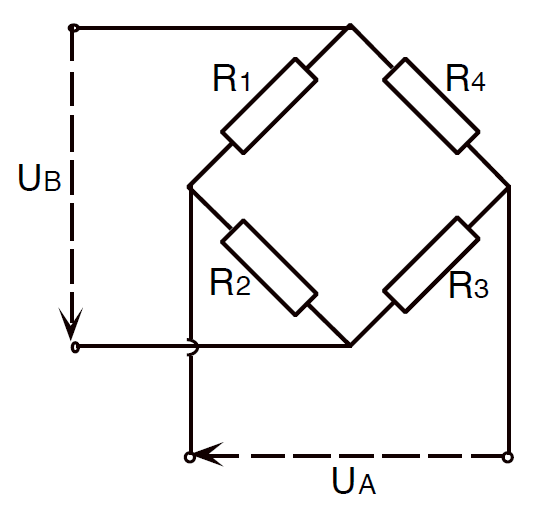
\includegraphics[width=.45\linewidth]{images/wheatstone_Bruecke}
	\caption{Wheatstone-Brücke}
	\label{fig:wheatstonebruecke}
\end{figure}
Wird eine Brückenspeisespannung $U_B$ angelegt, kann mit der Formel \ref{glg_U_A} $U_A$ berechnet werden\cite{Looser_Kraftmessung}. 

\begin{equation}\label{glg_U_A}
 U_A=\frac{R1 \cdot R3-R2 \cdot R4}{(R1+R2) \cdot (R3+R4)} \cdot U_B 
\end{equation}
Ist der Flex-Sensor dabei in Ruhelage, misst man eine Spannung von 0V. Aus dem Verhältnis von $ U_A $ zu $ U_B $ erhält man die relative Dehnung S des Flex-Sensors \todo{Quelle Prof. Dr. Herbert Looser, „M4 Kraftmesstechnik“, FHNW, 04.06.14}.
\begin{equation}\label{S_relativeDehnung}
S=\frac{U_A}{U_B}
\end{equation}
$U_A$ wird mit dem 10-Bit Analog- Digital-Wandler auf dem Mikrocontroller gemessen und mithilfe der fixen Spannung $U_B$ wird die relative Dehnung S berechnet. 


\section{Stromversorgung}
\label{HW_Stromversorgung}
An die Stromversorgung werden einige Anforderungen gestellt. So muss sie für die Motorsteuerung grosse Ströme mit bis zu 50A liefern können. Gleichzeitig muss die Spannung der Zellen kontinuierlich überprüft werden, um ein Tiefentladen zu verhindern. Zudem wird eine Standby-Killer Schaltung implementiert und dessen Funktion erklärt.\\
Um das Board einfach laden zu können ohne jedes Mal den Akku ausbauen zu müssen, hat sich das Team entschieden, eine Akku-Ladeschaltung einzubauen. Diese muss die Zellen balancen und sie vor Überspannung bzw. Überladung schützen. 
Im Folgenden wird das Balancing, die Ladeelektronik, die Selbsterhaltung, der verwendete Mikrokontroller und die Zellmessung genauer erläutert.
\subsection*{Balancing}
Das Balancing, wie man schon im Kapitel \ref{tGl_Balancing} erfahren hat, ist eine wichtige Funktion damit der Akku nicht zerstört wird. Das ganze Balancing sollte möglichst einfach aufgebaut sein und mit dem Mikrocontroller ansteuerbar sein. Wie man in Abbildung \ref{fig:Balancing} sieht, wurde dies mit einer P-Kanal MOSFET Schaltung ermöglicht. Der Widerstand am Drain des P-Kanal MOSFET reguliert den Strom mit welchem die einzelnen Zellen ausgeglichen werden. Damit die Schaltung mit einem Mikrocontroller gesteuert werden kann, brauch es einen N-Kanal MOSFET der das Gate des P-Kanal MOSFET auf Ground zieht. Mit dieser einfachen Schaltung ist es möglich die sechs Zellen des Akku zu balancen.

\begin{figure} [H]
	\centering
	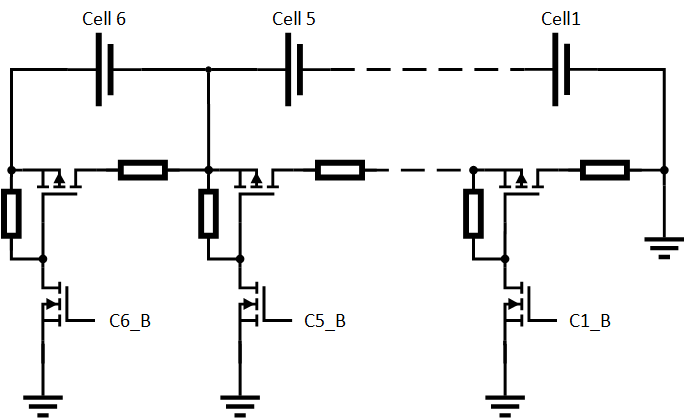
\includegraphics[width=0.6\linewidth]{images/Balancing}
	\caption{Balancing}
	\label{fig:Balancing}
\end{figure}




\subsection*{Ladeelektronik}
Damit der Akku fachgerecht geladen wird, braucht es eine Ladeelektronik, welche den Lipo-Akku nach dem CCCV-Verfahren lädt. Es gab zwei Möglichkeiten wie man dies hätte aufbauen können. Die eine Möglichkeit ist ein teures IC gewesen, welches auf dem Markt verfügbar wäre, die andere Möglichkeit ist eine günstige Buck-Converter Schaltung, mit welchem man auch nach dem oberen Verfahren laden kann. Ein solcher Buck-Converter kommt nun in diesem Produkt zum Einsatz

\begin{figure} [H]
	\centering
	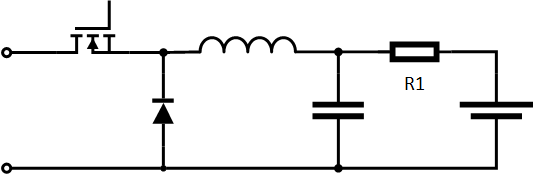
\includegraphics[width=0.6\linewidth]{images/Buck_Converter}
	\caption{Buck-Converter}
	\label{fig:Buck_Converter}
\end{figure}

Wie man in der vereinfachten Abbildung \ref{fig:Buck_Converter} des Buck-Converter sieht, ist dieser einfach und schnell aufgebaut. Der Widerstand R1 ist ein Shunt-Widerstand, an welchem der Strom gemessen wird. Anhand dieses Stromes wird der PWM, welcher über einen High-Side Treiber am Mosfet anliegt, durch den Mikrocontroller geregelt. Die Taktfrequenz des Clocks liegt bei 31.3kHz und wurde mit der Formel \eqref{eqn:Taktfrequenz} aus dem Datenblatt des Atmega berechnet.

\begin{equation}
f_{ PWM }=\frac { { f }_{ uC } }{ N*256 } 
\label{eqn:Taktfrequenz}
\end{equation}

Mit dieser Taktfrequenz kann man nun die grösse der Spule definieren. Dies wird mit folgender Formel \eqref{eqn:Spule} berechnet.

\begin{equation}
L=\frac { RF*\left( { V }_{ IN }-{ V }_{ OUT } \right) *\frac { { V }_{ OUT } }{ { V }_{ IN } }  }{ { f }_{ s }*{ I }_{ OUT } }  
\label{eqn:Spule}
\end{equation}

Berechnet wurde eine Spule von rund 120uH. Eingesetzt wurde eine Coilcraft-Spule mit dem Wert von 100uH. Da die Batterie wie ein grosser geladener Kondensator wirkt, sind keine all zu grossen Ripple am Ausgang des Buck-Converter zu erwarten.

\subsection*{Selbsterhaltung}
Wenn das Board voll geladen ist oder die fahrt für mehr als 20min unterbrochen wird, sollte es sich selbstständig herunterfahren und möglichst keinen Strom brauchen. Dafür wurde eine Selbsterhaltungsschaltung entwickelt (Abbildung \ref{fig:Selbsterhaltung}). Sobald beim Mikrocontroller einer von beiden Zustände eintrifft, wird der N-Kanal Mosfet ausgeschaltet. Somit wird die Speisung auf dem gesamten Print unterbrochen. Dadurch wird die Batterie bei einer längeren Lagerung vor dem zerstören geschützt.

\begin{figure} [H]
	\centering
	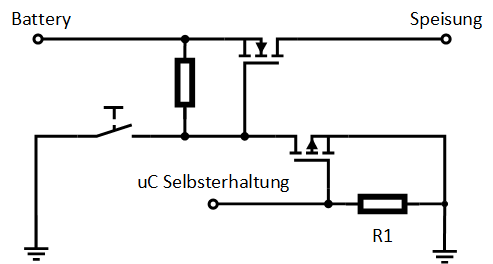
\includegraphics[width=0.6\linewidth]{images/Selbsterhaltung}
	\caption{Selbsterhaltung}
	\label{fig:Selbsterhaltung}
\end{figure}






\subsection*{Mikrocontroller}
Der Mikrocontroller muss verschiedene Anforderungen erfüllen.
In der folgenden Tabelle \ref{tabGPIObat} werden die General-Purpose-Input-Output-Anforderungen (GPIO-Anforderungen) an den Mikrocontroller aufgelistet.
\begin{center}
	\begin{tabular}{|c|c|c|c|}
		\hline 
		Beschreibung & Anforderung & Input/Output & Anzahl \\ 
		\hline 
		Überwachung der Zellen & Analog & Input & 6 \\ 
		\hline 
		Überwachen des Ladestroms &	Analog & Input & 1 \\ 
		\hline 
		Überwachen der Eingangsspannung & Analog & Input & 1 \\ 
		\hline 
		&  &  &  \\ 
		\hline 
		Entladen der Zellen (Balanceing) & Digital  & Output & 6 \\ 
		\hline 
		Anzeige des Ladezustands (LED) & Digital & Output & 3 \\ 
		\hline 
		Schalten des Ausgang Stroms zum Motor & Digital & Output & 1 \\ 
		\hline 
		Selbsthaltung des Mikrocontrollers & Digital & Output & 1 \\ 
		\hline 
		&  &  &  \\ 
		\hline 
		Regelung des Ladestroms & PWM & Output & 1 \\ 
		\hline 
		Kommunikation SPI Schnittstelle MISO/MOSI/SCK & Serial & In/Output & 3 \\ 
		\hline 
	\end{tabular} 
	\captionof{table}{GPIO Anforderungen für den Mikrocontroller}
	\label{tabGPIObat}
\end{center}
Für die Regelung der Stromversorgung wird der Mikrocontroller ATmega328P-AU verwendet.
\subsection*{Zellmessung}
Für das bessere Verständnis der Zellmess-Schaltung wird die Entwicklung geschildert. \\
Das Ladegerät besteht aus jeweils sechs Zellen, die in Serie geschaltet sind, um dem Motor genügend Spannung zur Verfügung zu stellen. Mit einer Zellenspannung von 4.15V pro Zelle liegt am obersten Punkt (Anode der Zelle 6) eine Spannung von 24,9V an. Da die Spannung an den Eingängen des Mikrocontrollers nicht seine Speisespannung übersteigen sollte, mussten diese Spannungen verringert werden. Für den verwendeten Mikrocontroller beträgt die maximale Spannung am Eingang 5V.
\\
Die einfachste Variante ist, mit einem Spannungsteiler die Spannungen so skaliert, dass die Maximalspannung nicht überschritten wird. Diese Grundschaltung ist in Abb.\ref{fig:zellmessung} links oben zu sehen. 
\begin{figure} [H]
	\centering
	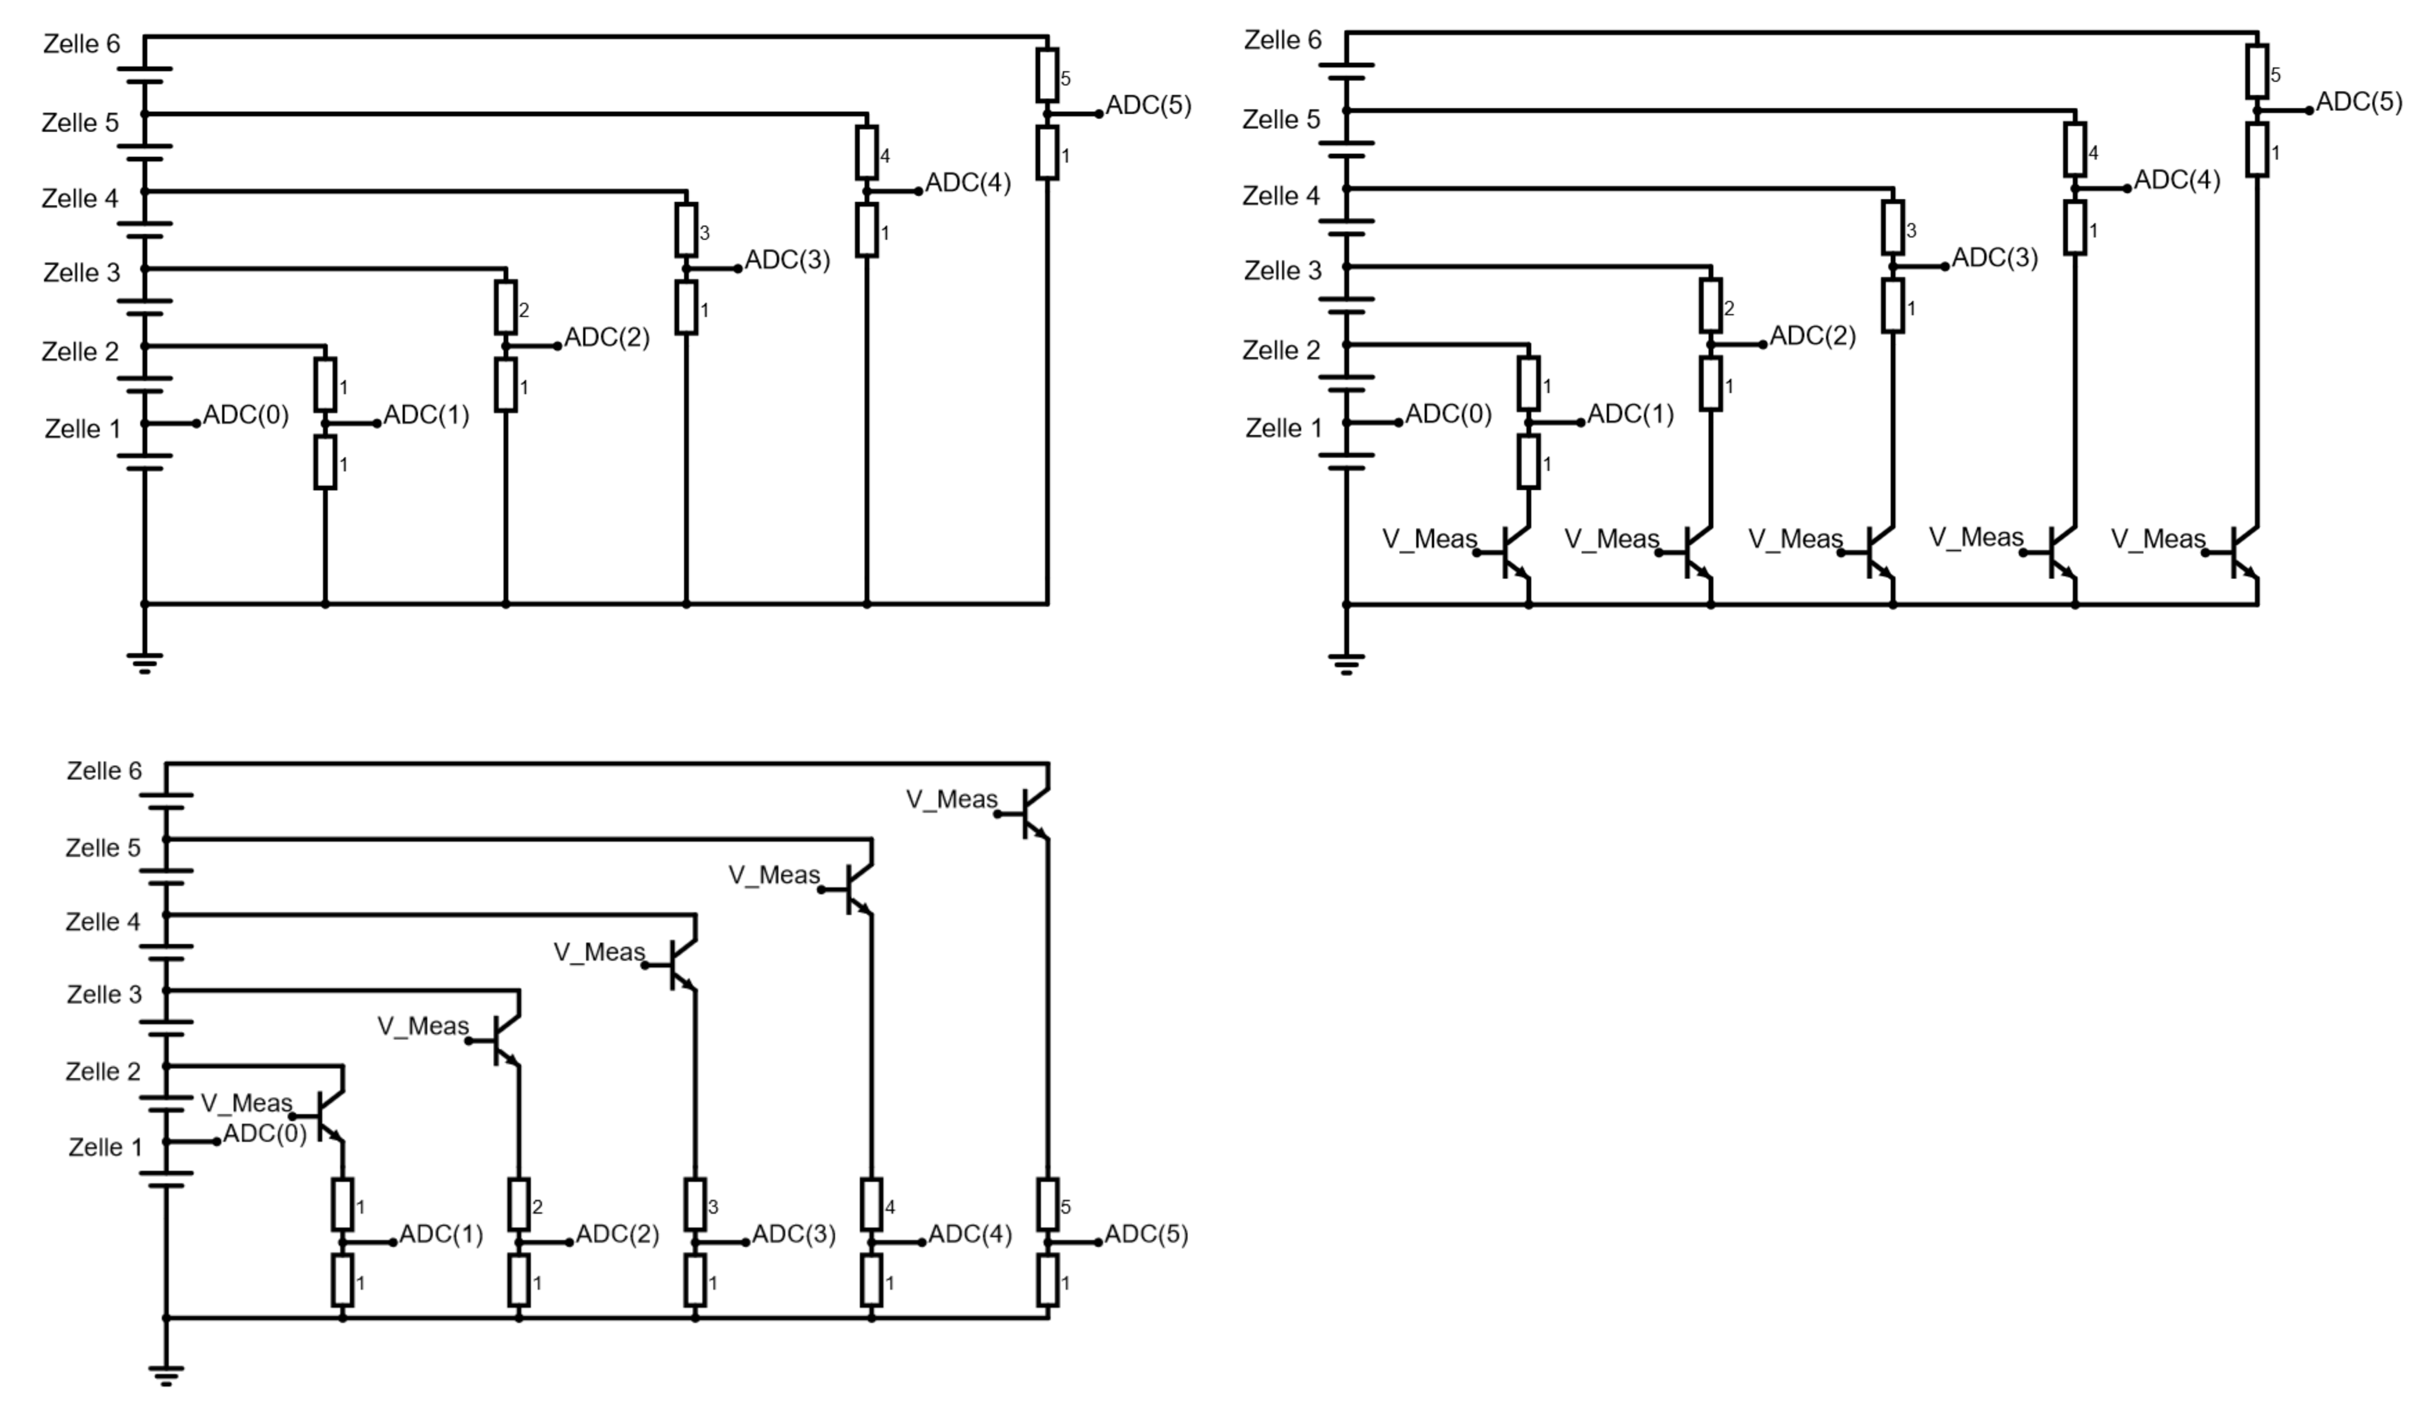
\includegraphics[width=1\linewidth]{images/Zellmessung}
	\caption{Messung der Zellen - drei Messschaltungen}
	\label{fig:zellmessung}
\end{figure}
\todo{besserer Titel für Abb.}
\todo{a b c bzw Var 1, Var 2, Var3 fürs Bild...}
Der Nachteil dieser Schaltung ist, dass die Zellen durch die Spannungsteiler kontinuierlich entladen werden. Somit können bei einem längeren Nichtgebrauch die Akkuzellen entladen oder sogar tiefentladen sein. \\
Um dies zu verhindern, wurde die Schaltung mit Transistoren erweitert (Abb.\ref{fig:zellmessung}). Diese Transistoren unterbrechen den Entladestromkreis über den Widerständen. Dazu werden die Transistoren übersteuert, um sie als Schalter zu verwenden und den durch die Sättigungsspannung $U_{CE}$ entstehende Fehler zu verkleinern. Dieser kann jedoch je nach Sättigungsspannung der Transistoren und aufgrund der unterschiedlichen Bauarten nur schwer korrigiert werden. Der zweite grosse Nachteil (und gleichzeitig das Killerkriterium für diese Schaltung) ist, dass durch das Unterbrechen des Spannungsteiler-Stromkreises an den ADC-Ausgängen wieder die Zellenspannung anliegt. Dadurch würden sich die Zellen über die Ableitdiode am Eingang des Mikrocontrollers entladen und diese Diode voraussichtlich zerstören. \\
Dies könnte verhindert werden, indem der Stromkreis oberhalb der ADC-Eingängen unterbrochen wird. Dies ist in der linken unteren Schaltung der Abb.\ref{fig:zellmessung} gezeichnet. Dadurch wären die Eingänge vor Überspannung geschützt. Aber auch diese Schaltung enthält diverse Nachteile. So fliesst beim geschlossenen Zustand der Basis-Emitter-Strom durch den Spannungsteiler. Dies verfälscht die Messresultate. Zusätzlich muss zwischen Basis und Emitter eine Schaltspannung von mindestens 0.7V anliegen. Dazu müsste die Schaltspannung 0.7V über der Zellspannung liegen, was nur mit grossem Aufwand erreichbar wäre. 
Das Team entschied, die erste Methode zu wählen, da sie die genausten Messungen liefert und die Entladung der Zellen bei einer durchschnittlichen Benutzung des Boards nicht problematisch ist, also keine Tiefentladung auftritt.

\section{Motoransteuerung}
\label{HW_Motoransteuerung}
Die Motoransteuerung ist bei der angetriebenen Achse montiert. Die Funktion deser Steuereinheit wird im folgenden im Überblick kurz erläutert und danach wird auf die einzelnen Bestandteile eingegangen.
Bei diesem Board kommt die Drehfeldanregung mit FOC (Field Oriented Control) zum Einsatz, was bedeutet, dass die drei Phasen mit drei, jeweils um 120\(^\circ\) phasenverschobene, Sinusströmen bestromt werden. Dies erzeugt ein rotierendes Drehfeld, welches den aus Permanentmagneten bestehenden Erregerkreis auf dem Rotor mit einem Drehmoment versieht. Dieser grundsätzliche Ablauf wird hardwaretechnisch so umgesetzt:
In einem \textbf{Mikrokontroller}, wird pro Motorphase ein PWM-Signal erzeugt, welches integriert und gemittelt ein Sinussignal ergibt. Über einen intelligenten und schnellen \textbf{Treiber} werden dann die in einer H-Brücke angeordneten N-Kanal \textbf{MOSFET Transistoren} angesteuert, welche dieses PWM-Signal dann mit grosser Leistung an die Klemmen geben. Da jede Phase im Motor eine Spule ist, und der Strom durch eine Spule das Integral der Spannung ist, ergibt sich so dieser quasi-sinusförmige Stromverlauf.
An zwei Phasen werden die Ströme über Shunt-Messwiderstände gemessen und dem Mikrokontroller über einen A/D-Wandler mitgeteilt. Dies ist dann die Grundlage für die integrierte Regelung.

\subsection*{Mikrokontroller}
Verwendet wird der Mikrokontroller STM32F303, dies weil es ein bewährter und bekannter Mikrokontroller ist, der mit seinen 8MHz Taktfrequenz genügend schnell ist. Dazu unterstützt er die PWM Funktion, hat genügend I/O-Ports und bleibt preislich im Budget.
An ihm wird über ein SPI Interface noch das HopeRF RFM75 Modul angeschlossen, welches mit der Steuerung, dem Magic Glove, über eine 2.4 GHz-Funkverbindung kommuniziert.

\begin{tabularx}{\textwidth}{l|l|l|X}
	Typ & Pins & Ports & Beschreibung \\ \hline
	Analog & 
	11,14-16,26-27 & 
	A, B, C &
	Analoge Eingänge zur Messung der Phasenströme und -Spannungen sowie der Versorgungsspannung.
	\\ \hline
	Digital & 
	54-56,37-38 &
	B, C, D &
	Standard digitale Steuersignale zum und vom Treiber-IC. Statussignale für Fehlermeldungen (FAULT, OCTW, PWRGD) und Steuersignale (EN\_GATE, DCCAL).
	\\ \hline
	SPI &
	50-53 &
	A, C &
	SPI Bus zum Treiber-IC für Einstellungen und Statusmeldungen.
	\\ \hline
	PWM &
	34-36, 41-43 &
	A, B &
	PWM Signale für die Halbbrücken. Diese gehen an das Treiber-IC, welches die FETs ansteuert.
	\\ \hline
	Digital &
	8,10 &
	C &
	Steuersignale IRQ und Chip-Enable für das RFM-Modul.
	\\ \hline
	SPI &
	51-53, 9 &
	C &
	SPI Bus zum RFM-Modul. Die Datenleitungen SDI und SDO sowie die Taktleitung SCK werden mit dem Treiber IC geteilt. Es unterscheiden sich nur die Chip-Select-Signale.
	\\ \hline
	UART &
	29,30 &
	B &
	Serielle Schnittstelle zu Debug-Zwecken. Wird nur in der Entwicklung verwendet.
	\\ \hline
	SWD &
	7, 46,49 &
	A &
	Programmierschnittstelle
	\\ \hline
	USB &
	44,45 &
	A &
	USB Schnittstelle vorgesehen, wird jedoch nicht verwendet.
	\\ \hline
\end{tabularx}
\captionof{table}{Ein-/Ausgänge Mikrocontroller}
\label{tab:iomc}

\subsection*{Endstufe (Treiber und H-Brücken)}
Für die Ansteuerung Transistoren wird der DRV8301 Gate-Treiber von Texas Instruments verwendet. Dieser Treiber beinhaltet einen Gate Driver mit 1.7A Peak Gatestrom, Current Shunt Differenzverstärker, Über- und Unterspannungsschutz sowie Übertemperaturschutz und Überstromschutz. Ebenfalls ist ein Buck Converter für die Spannungsversorgung eingebaut.
Die Transistoren sind IRFS7534 N-Kanal Power MOSFETs von Infineon, die 60V und 164A permanent aushalten. Sie eignen sich besonders für schnelles Schalten von grossen Lasten, also genau dieses Einsatzgebiet. Dies vor allem wegen dem tiefen $R_DSon$ (typ. 2\(\Omega\)) und der geringen Eigenkapazität. 
Für die Ansteuerung Transistoren wird der DRV8301 Gate-Treiber von Texas Instruments verwendet. Dieser Treiber beinhaltet einen Gate Driver mit 1.7A Peak Gatestrom, Current Shunt Differenzverstärker, Über- und Unterschutzspannung sowie Übertemperaturschutz und Überstromschutz. Ebenfalls ist ein Buck Converter für die Spannungsversorgung eingebaut.
Die Transistoren sind IRFS7534 N-Kanal Power MOSFETs von Infineon, die 60V und 164A permanent aushalten. Sie eignen sich besonders für schnelles Schalten von grossen Lasten, also genau dieses Einsatzgebiet. Dies vor allem wegen dem tiefen $R_{DSon}$ (typ. 2\(\Omega\)) und der geringen Eigenkapazität. 

\subsection*{Messschaltungen}
In der Ansteuerung von zwei Phasen sind 0.1\(\Omega\) Shunt-Widerstände zur Strommessung eingebaut. Die Spannung über den Widerständen wird im Gate-Treiber um den Faktor 10 verstärkt und mit einem Offset von $\frac{V_{logic}}{2}$ versehen. Der Mikrocontroller erhält dann eine Spannung zwischen 0 und $V_{logic}$ von dem Treiber. Damit wird dann der dritte Phasenstrom berechnet und dann zur Regelung verwendet.
